The lab assignments under-specifies the operation of virtual-indexed caches, as
it does not specify what method to use to avoid aliasing (having multiple
entries in the cache for the same physical address, if it's represented by
multiple virtual addresses).

My implementations do the following when a new block is brought into the cache:
\begin{itemize}
  \item The virtually-indexed physically-tagged cache checks the tags in all
  the cache lines that could potentially hold the virtual address (one line for
  small caches, more lines for large caches), and invalidates any location that
  has the same tag.
  \item The virtually-indexed virtually-tagged cache checks the physical bits
  in the tags (could be zero bits, if the cache is big enough) against the
  physical bits in the new block's address, and invalidates all the blocks
  whose bits match.
\end{itemize}

Implementation note: I rewrote the testing script to be able to test different
pintools (or the same pintool with different parameters) in parallel. I removed
the parallelization bottleneck which was using a statically-named temporary
directory. I also fixed the results oudirectory permissions bug (the original
script used 666, which makes the results directory non-browsable on systems
that actually obey the permission bits, which is everything except AFS). Last
but not least, my testing tool is driven by configuration files. I checked in
the tool (\texttt{./pin\_spec.rb}) as well as my configuration files
(\texttt{pin\_spec.yml}, \texttt{spec\_suite.yml}, and \texttt{tests/1.yml} -
\texttt{tests/22.yml}).

My results were produced using 10 computers in an Athena cluster over 5 hours.
About 20 CPU-hours were wasted due to bugs at various levels, and the results
of the other 30 hours made it into this paper. I used the cluster during
off-peak hours.

\section{Question 1}
The lab handout is unclear about the desired way of varying the parameters. I
changed one parameter (number of rows, block size, associativity) while keeping
the other parameters constant. I only increased (as opposed to decreasing) the
parameters because the default parameters yield a cache size of 2kb, and today's
L1 caches are bigger.

I compared caches of the same size, obtained by increasing one of the
parameters from the basic configuration. The graphs have the 3 caches and
initial configuration as the baseline. Graphs show cache misses, so lower lines
indicate better performance.

Figures \ref{q1:4k}, \ref{q1:8k}, \ref{q1:16k}, and \ref{q1:32k} show the
results.

\begin{figure}[htb]
  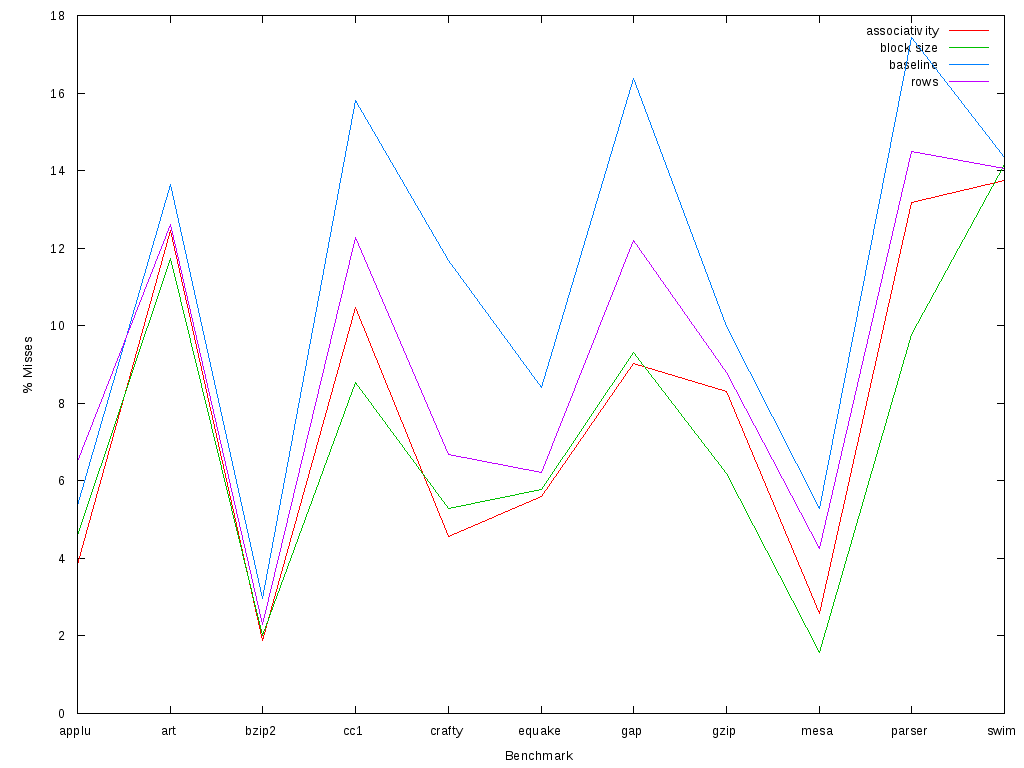
\includegraphics[width=6.8in]{6.823/lab2/figs/ccc_4k.png}
  \caption{Miss rates in 4kb caches obtained by increasing a parameter
  (number of rows, block size, associativty) from a baseline 2kb direct-mapped
  cache with 4-byte blocks.} \label{q1:4k}.
\end{figure}

\begin{figure}[htb]
  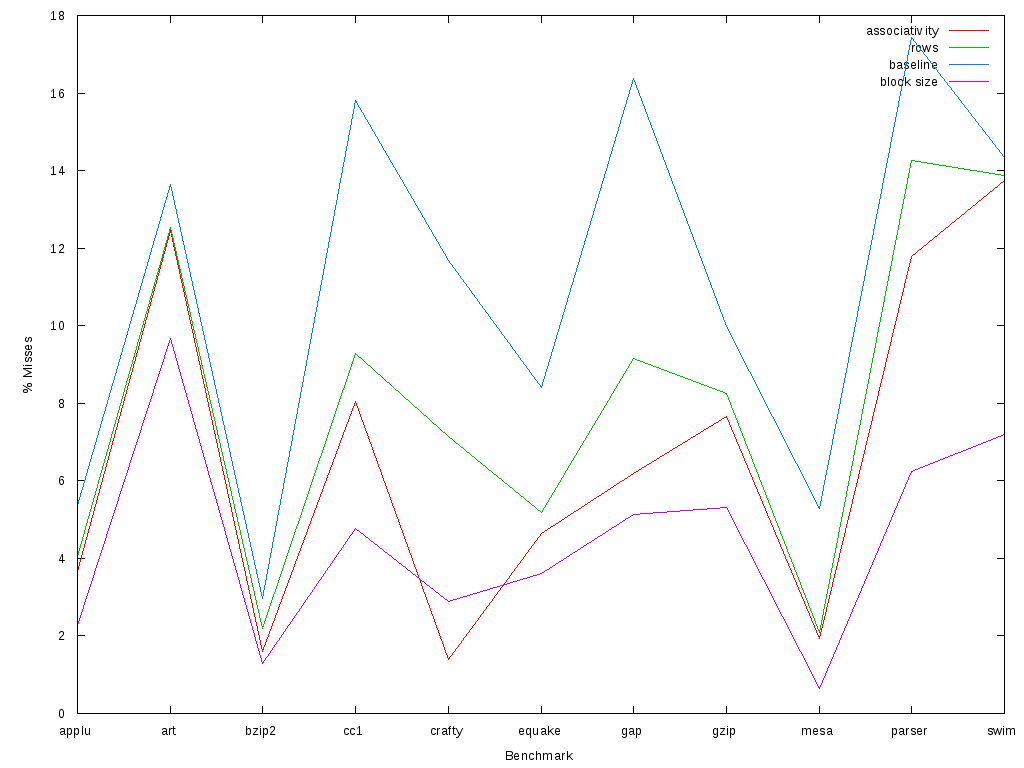
\includegraphics[width=6.8in]{6.823/lab2/figs/ccc_8k.png}
  \caption{Miss rates in 8kb caches obtained by increasing a parameter
  (number of rows, block size, associativty) from a baseline 2kb direct-mapped
  cache with 4-byte blocks.} \label{q1:8k}.
\end{figure}

\begin{figure}[htb]
  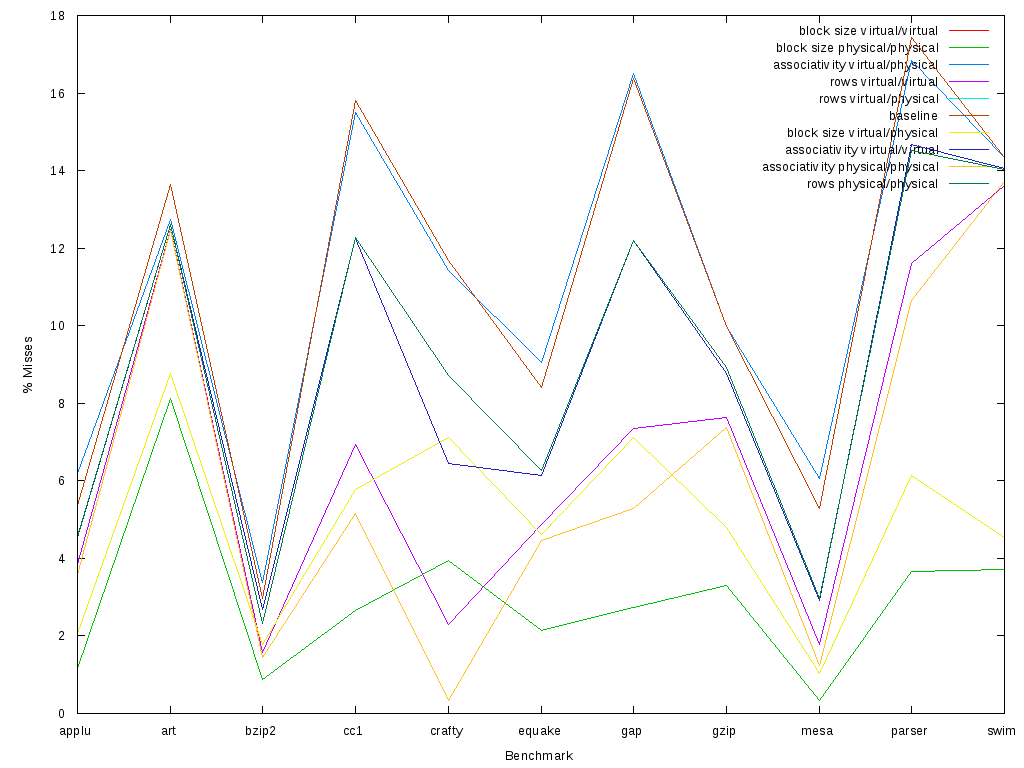
\includegraphics[width=6.8in]{6.823/lab2/figs/ccc_16k.png}
  \caption{Miss rates in 16kb caches obtained by increasing a parameter
  (number of rows, block size, associativty) from a baseline 2kb direct-mapped
  cache with 4-byte blocks.} \label{q1:16k}.
\end{figure}

\begin{figure}[htb]
  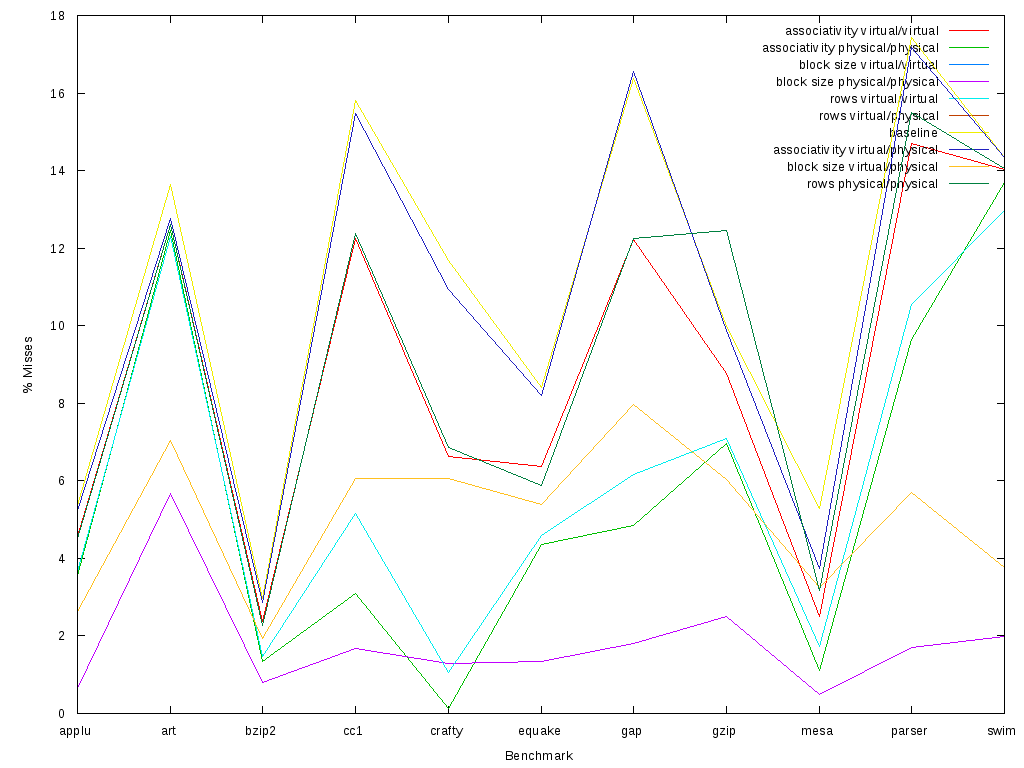
\includegraphics[width=6.8in]{6.823/lab2/figs/ccc_32k.png}
  \caption{Miss rates in 32kb caches obtained by increasing a parameter
  (number of rows, block size, associativty) from a baseline 2kb direct-mapped
  cache with 4-byte blocks.} \label{q1:32k}.
\end{figure}

The best way of reducing cache misses, for small caches, seems to be to
increasing the block size, which reduces compulsory misses. This is not
surprising, because the conclusion is in line with the course textbook, and
with today's manufacturers' decisions to use 32-byte blocks.

Increasing the block size becomes less desirable once the block size passes 32
bytes, and compulsory misses are starting to become dominated by conflict and
capacity misses. Caches with higher associativity dominate caches with higher
row counts, but the difference isn't very big, which suggests that
set-associative caches are not worth the extra latency they would add to an L1
cache. Again, this is in line with previous findings.

Last, caches with physical indexing show a significantly better hit rate than
caches with virtual indexing. However, once virtual indexing is employed, it
seems that there's no big difference between virtual tagging and physical
tagging. On the sad side, the cache simulation seems to have a bug because, in a
couple of cases, virtually-tagged caches seem to perform better than
physically-tagged caches, which is pretty much impossible.

\section{Question 2}
To determine the working set sizes, I used direct-mapped caches with the
minimum block size (4 bytes). I stopped at a cache size of 512kb because 
higher values made the \texttt{caches} pintool really slow, and the simulations
did not finish in time to be included in this report.

Figure \ref{q2:miss_rates} shows the miss rates. Table \ref{q2:working_set}
shows the probable working set sizes, based on the miss rates obtained above.

\begin{figure}[htb]
  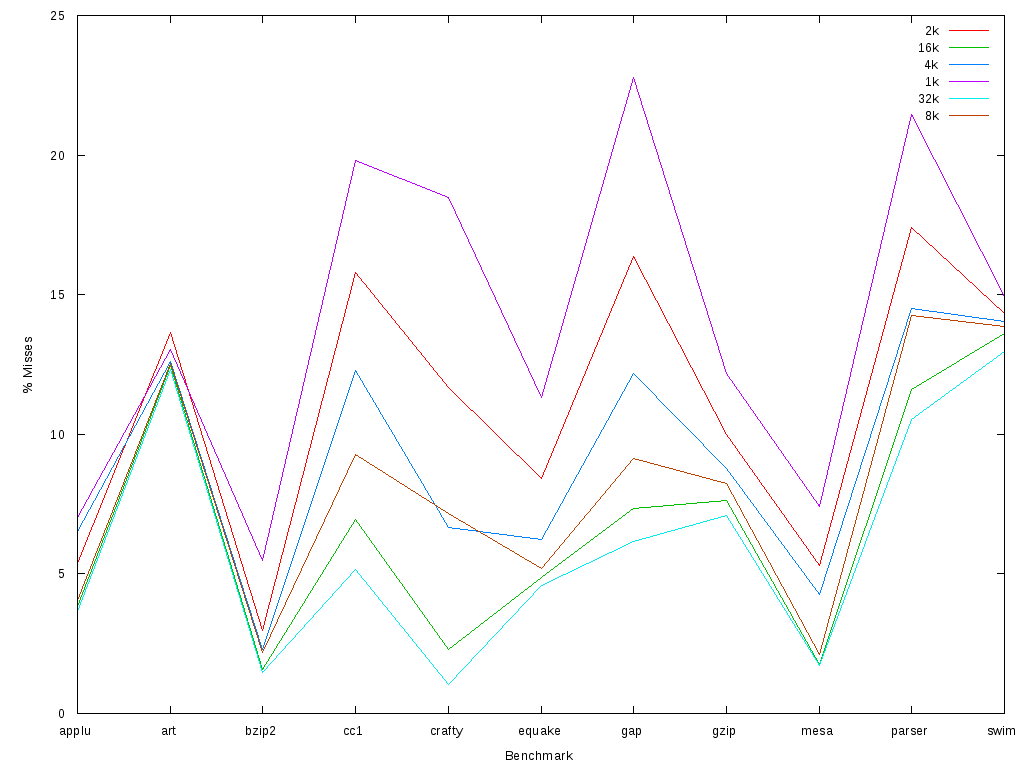
\includegraphics[width=6.8in]{6.823/lab2/figs/working_set.png}
  \caption{Miss rates in direct-mapped physically-indexed physically-tagged
  caches with 4-byte blocks. }
  \label{q2:miss_rates}.
\end{figure}

\begin{figure}[htb]
\center

\begin{tabular}{lcr}
\hline
Benchmark & Integer / FP & Working set size \\
\hline
bzip2 & INT & 32kb \\
cc1 & INT & $>$ 512kb \\
crafty & INT & 512kb \\
gap & INT & $>$ 512kb \\
gzip & INT & $>$ 512kb \\
parser & INT & $>$ 512kb \\
\hline
applu & FP & $>$ 512kb \\
art & FP & $>$ 512kb \\
equake & FP & 64kb \\
mesa & FP & 64kb \\
swim & FP & $>$ 512kb \\
\hline
\end{tabular}

\caption{The working set sizes for the SPEC 2000 benchmark suite. }
\label{q2:working_set}
\end{figure}

Both the integer and the floating point benchmarks have a mix of small
(around 64kb) and large work sets (greater than 256kb). An interesting case is
\texttt{bzip2}, which uses a lot of memory (I know that, because I know how the
Burrows-Wheeler transform works), but also has very good cache locality.
Integer benchmarks seem to have bigger worksets, based on the fact that miss
rates still drop significantly as the cache size goes to 256kb / 512kb. All
benchmarks have working sets that exceed the L1 caches of 2000 (around 4kb, if
memory serves me well), but some of them fit snuggly in L2 caches, which used
to be around 64-128kb (again, quoted from memory).

\section{Question 3}
The fourth cache model doesn't make any sense. The different cache models in
this lab are motivated by the desire of parallelizing cache access and address
translation.

If the cache is physically indexed, it means the cache access cannot start unil
after address translation. Since we waited for address translation anyway, we
might as well use the physical address for the tag. There's no reason to deal
with the additional complexities of using virtual tagging.

\section{Question 4}
Having more than one process at a time means that each process will have its
own page tables, and therefore the virtual-to-physical mapping can change
during cache operation.

The physically-indexed physically-tagged cache isn't impacted by this change at
all, since it's oblivious to address translation.

The virtually-indexed physically-tagged cache is equipped to deal with this
change. If the mapping changes, the tag will not match, so the cache will not
give a bad answer by mistake. The cache's design has to deal with aliasing
(different virtual addresses pointing to the same physical address) for the
single-process case, so multiple processes don't introduce a change.

The virtually-indexed virtually-tagged cache cannot function correctly with a
naive implementation. Process ID bits will have to be added to the tag bits. On
the bright side, the process ID bits count as physical tag bits, which allows
for bigger associative caches. Clarification: in a virtually-indexed,
virtually-tagged cache, the physical bits of the tag are the bits that belong
to the page offset, and therefore will not be changed by address translation.
The number of physical tag bits determines the maximum associativity of the
cache. For example, a 4-way associative cache is useless with 1 physical tag
bit, because a row will never have all its 4 ways filled.

For the 512-bytes cache with 256-bytes pages, all the physically-tagged
combinations will work (with better or worse results). The virtually-tagged
cache model can't be implemented. A $2^n$-row $2^b$-byte block cache would have
$8 - n - b$ physical tag bits. However, the same cache needs to have
$\frac{512}{2^n \cdot 2^b} = 2^{9 - n - b}$ ways, so there aren't enough
physical tag bits for a virtually-indexed virtually-tagged cache.

The TAs would have to modify the address translation routine in our source code
to simulate different processes, so I doubt that will be part of the tests. 

\section{Question 5}

I stripped the supplied \texttt{caches} pintool into a pintool that counts the
read and write memory accesses, as well as the aligned reads and writes. The
summaries are presented in figure \ref{q5:unaligned_accesses}.

\begin{figure}[htb]
\center
\begin{tabular}{lrrr}
\hline
Test & \% unaligned reads & \% unaligned writes & \% unaligned accesses \\
\hline
applu & 0.00019\% & 0.00047\% & 0.00023\%  \\
\hline
art & 0.00013\% & 0.00050\% & 0.00019\%  \\
\hline
bzip2 & 0.24491\% & 0.36827\% & 0.28971\%  \\
\hline
cc1 & 0.04994\% & 0.01413\% & 0.03852\%  \\
\hline
crafty & 0.02442\% & 0.01042\% & 0.01913\%  \\
\hline
equake & 0.01114\% & 0.01851\% & 0.01239\%  \\
\hline
gap & 0.08745\% & 0.04416\% & 0.07358\%  \\
\hline
gzip & 0.14022\% & 0.12515\% & 0.13500\%  \\
\hline
mesa & 0.07836\% & 0.08633\% & 0.08100\%  \\
\hline
parser & 0.07013\% & 0.00846\% & 0.04782\%  \\
\hline
swim & 0.00003\% & 0.00007\% & 0.00004\%  \\
\hline
{}Averages & 0.06426\% & 0.06150\% & 0.06342\%  \\
\hline
\end{tabular}

\caption{The percentage of unaligned memory accesses out of the total memory
accesses for the SPEC 2000 benchmark suite. }
\label{q5:unaligned_accesses}
\end{figure}

The bulk of unaligned accesses come from \texttt{bzip2}, which is a compression
tool, and therefore it works with streams of bytes. Other significant sources
of unaligned accesses are also processing streams of bytes -- \textt{cc}
compiles C code, and \textt{parser} presumably builds an AST out of some
language. The one that didn't come to my mind was \texttt{mesa}, which is
(hopefully, if my guess is right) a software OpenGL implementation, and
therefore has to work with a software framebuffer.

The assumption of aligned accesses seems to make sense for most benchmarks. The
numbers reported above are an upper bound of unaligned accesses because, from a
cache perspective, byte accesses can be satisfied even if they're unaligned, and
multibyte accesses are only problematic if they span across 2 cache blocks.
Furthermore, the applications which are most impacted by unaligned access don't
really run on consumer computers -- most people don't compile their code, and a
vast majority of desktop and mobile platforms have accelerated graphics
nowadays.
